\chapter{\label{chap:problem}O Problema}
Estabelecer a complexidade computacional de jogos -- sejam jogos de carta,
jogos de tabuleiro ou jogos digitais -- é uma prática muito importante e comum.
Através desta categorização, obtemos evidências do porquê humanos consideram
estes problemas interessantes, além de indicar para pesquisadores da área os
desafios propostos vistos de uma perspectiva de tarefa de otimização.  Dados os
desafios presentes em Spelunky conclui-se que, computacionalmente falando,
trata-se de um problema, no melhor dos casos, do conjunto \textit{NP-Hard}
\cite{SPELUNKYHARD}.

O ambiente em Spelunky é \textbf{contínuo}, \textbf{parcialmente observável},
\textbf{dinâmico}, \textbf{estocástico} e \textbf{sequencial}. Estas
características influenciam fortemente na dificuldade do problema proposto pelo
jogo. Somado a isto, os níveis são gerados proceduralmente, cortando a
possibilidade de memorização do mapa. Contudo, o algoritmo utilizado para gerar
os níveis garante que existe pelo menos um caminho transponível do início ao fim
-- mesmo que com inimigos e armadilhas no caminho --, sem que seja necessário o
uso de bombas ou cordas para ajudar com desobstrução e locomoção. O personagem
tipicamente entra no nível pela parte superior e deve encontrar a saída que se
encontra na parte inferior do mapa. Um exemplo de geração de mapa pode ser
observado a seguir:

\begin{figure}[htb!]
\centering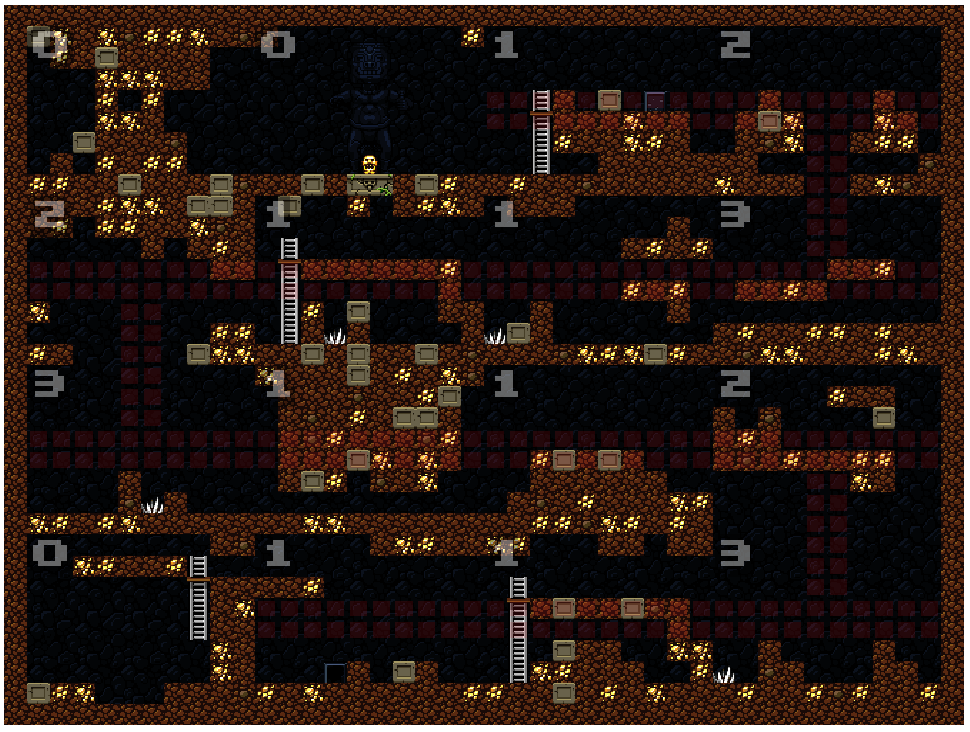
\includegraphics[width=.65\textwidth]{fig/spelunky-level-example.png}
\caption {\label{fig:spelunky-level-example}Exemplos de níveis gerados
proceduralmente.} \end{figure}

Outro agravante é o número de ações -- e combinações de ações -- que podem ser
executadas pelo jogador a cada atualização do jogo. Algumas delas são
influenciadas por itens equipados ou estado atual do jogador, o que significa
que, caso não se tenha o devido cuidado, podem gerar resultados inesperados,
resultando na perda de vida ou até mesmo no fim do jogo.

Os pontos de vida são o recurso mais importante do explorador, pois quando
esgotados, encerra-se a partida. Existem inúmeras maneiras de se perder este
recurso em Spelunky, como inimigos, armadilhas ou até mesmo uma queda de um
lugar muito alto.

A proposta desse trabalho é realizar a criação de \textit{bots} capazes de
jogar uma partida de Spelunky da melhor maneira possível, avaliando a
qualidade destes através de métricas como pontuação obtida e tempo de jogo.
Para auxiliar nesta tarefa, utilizar-se-á o \textit{framework} SpelunkBots.
Esta ferramenta comunica-se diretamente com o jogo, possibilitando a aquisição
de informações do ambiente -- como localização de inimigos, armadilhas e
tesouros --, o envio de ações para o explorador, entre outras facilidades --
algumas mencionadas anteriormente.
